\graphicspath{{chapt_dutch/}{intro/}{chapt2/}{chapt3/}{chapt4/}{chapt5/}}

% Header
\renewcommand\evenpagerightmark{{\scshape\small Chapter 4}}
\renewcommand\oddpageleftmark{{\scshape\small Event Simulation and Reconstruction}}

\hyphenation{}

\chapter{Event Simulation and Reconstruction}
\label{ch4}

In order to 2 addditional tools? are needed.

\section{Event generation}

\section{Detector simulation}

\subsection{Delphes}

\subsection{GEANT4}

\section{Event reconstruction}

\subsection{Track reconstruction}

The tracks of charged particles going through the \ac{CMS} tracker are reconstructed with an iterative tracking approach. This is used to cope with the high occupancy and consequently high combinatorics. Additionally, the first iterations search for tracks with less possible combinations, such as tracks with many pixel hits or a high momentum. After every iteration, the hits associated with the found track are removed to reduce the combinatorics. Each iteration consists of four steps:
\begin{enumerate}
 \item \textbf{Seed generation.} In this first step hits are combined into seeds for the subsequent track finding. In the initial iterations pixel triplets are used, then pixel pairs, in order to take gaps or non-working modules into account. Next, mixed pixel/strip triplets are taken, and finally strip-only seeds are used. These additional iterations improve the acceptance in $p_T$ and in displacement with respect to the primary vertex.
 \item \textbf{Track finding}. The seeds are used as starting point for a Kalman filter algorithm. This method extrapolates the seed trajectory outward to the next layer, taking into account potential energy loss and multiple scattering. If compatible hits are found in the next layer, the parameters of the trajectory are updated. This process continues until the outermost layer of the tracking system. Using this method, a given seed can generate multiple tracks, or different tracks can share hits. A trajectory cleaner therefore determines the fraction of hits the tracks have in common and discards the track with the lowest number of hits when there are too many shared hits. If both tracks have the same number of hits, the track with the largest $\chi^2$ value is removed.
 \item \textbf{Track fitting.} The track parameters are then refitted using a Kalman filter and smoother, taking all hits determined in the track finding step into account.
 \item \textbf{Track selection.} Finally, the tracks are selected based on quality requirements, such as the number of layers that have hits, the $\chi^2/$dof, and the distance to a primary vertex. This greatly reduces the fraction of reconstructed tracks that are fake.
\end{enumerate}

The performance of the track reconstruction is excellent, and a high track-finding efficiency is obtained~\cite{Chatrchyan:2014fea} while keeping the rate of fake tracks negligible. The highest tracking efficiency is obtained for muons, which traverse the full detector volume and have an improved momentum resolution due to tracking information from the muon detectors giving a long lever arm. For isolated muons with $p_T$ between 1 and \SI{100}{GeV} the tracking efficiency is higher than 99\% for the entire $\eta$ coverage of the tracker, as can be seen from the left plot in Figure~\ref{fig:eff_eta}. The $p_T$ resolution is about 2-3\% for a muon with $p_T = $ \SI{100}{GeV} up to $|\eta| < 1.6$, but worsens for higher pseudorapidities. Different types of particles interact differently with the detector material. Charged hadrons, for example, are also subject to elastic and inelastic nuclear interactions and have a tracking efficiency of 80-95\% depending on pseudorapidity and transverse momentum, as shown in the right plot of Figure~\ref{fig:eff_eta}.

\begin{figure}[ht]
  \centering
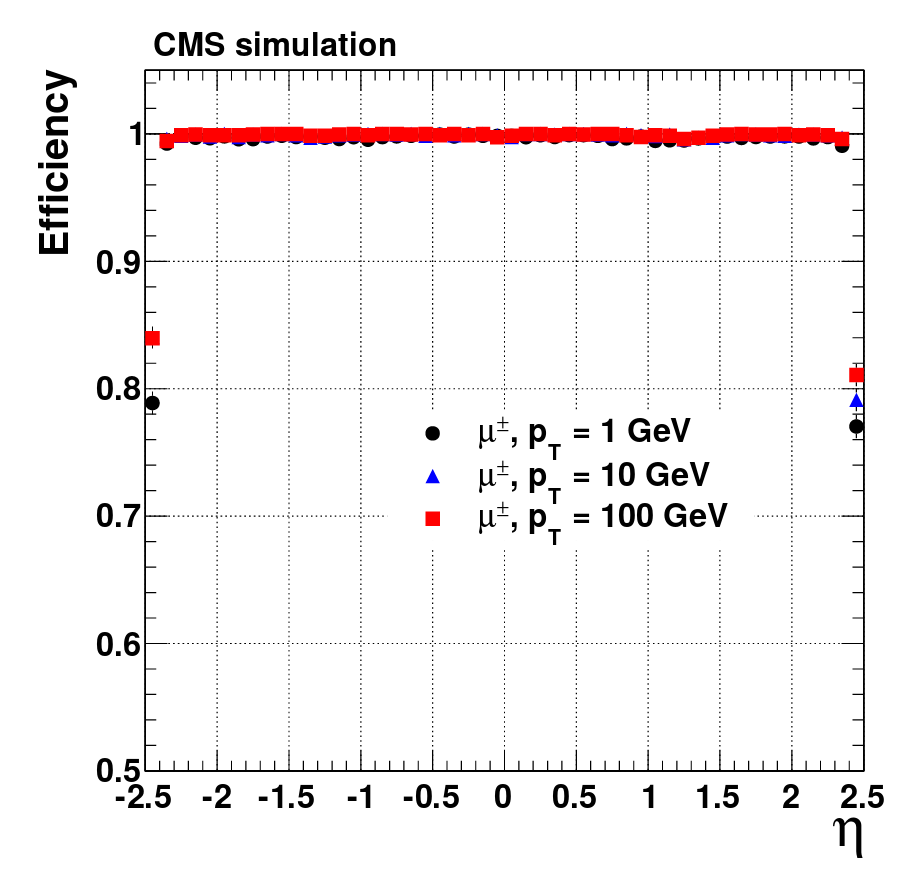
\includegraphics[width=.4\textwidth]{muon_eff_eta}\hspace{1cm}
 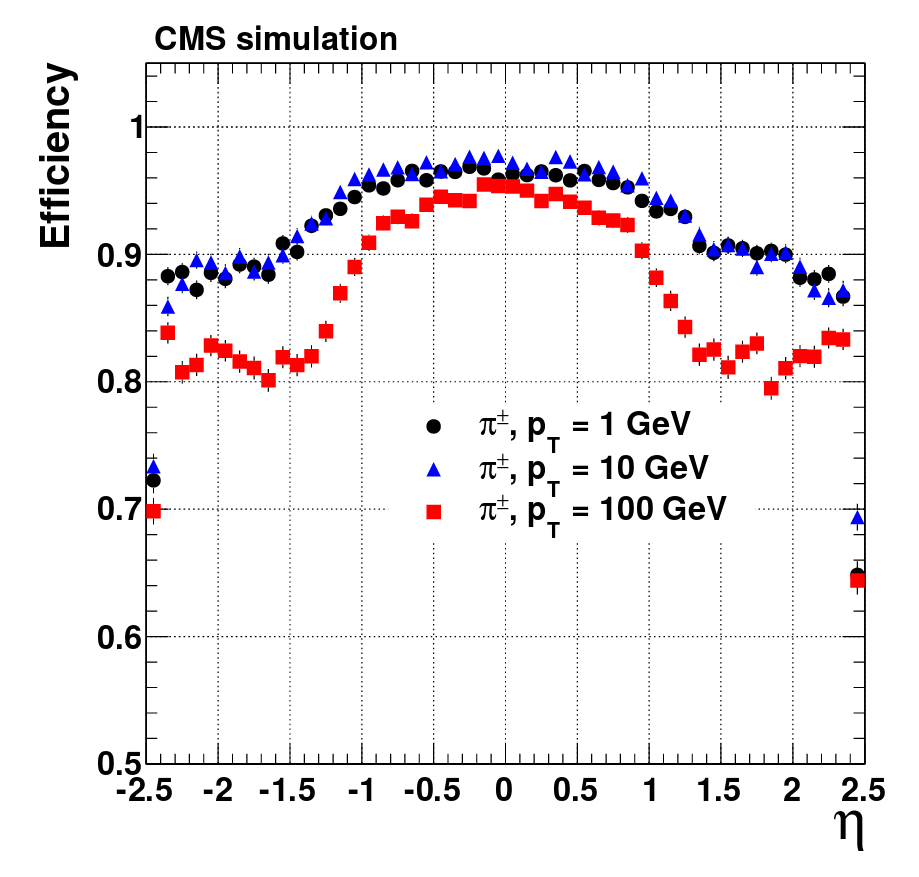
\includegraphics[width=.4\textwidth]{pion_eff_eta} 
 \caption{The muon efficiency (left) and pion efficiency (right) as a function of pseudorapidity, for multiple transverse momenta.~\cite{Chatrchyan:2014fea}}
 \label{fig:eff_eta}
\end{figure}

Finally, the primary vertex is reconstructed from the tracks. Since the collisions happen between bunches of protons, multiple protons will be colliding at the same time. The extra collisions, next to the potentially interesting collision, are referred to as pile-up interactions. The particles generated in these collisions are all detected simultaneously and form a challenge to disentangle them from the particles coming from the to be studied interaction.

The reconstruction is done in 2 steps: first the tracks that appear to originate from the same interaction vertex are clustered, then a fitting procedure computes the vertex parameters and assigns a weight to each associated track, reflecting the probability that it corresponds to the considered vertex. Figure~\ref{fig:PV} shows the reconstruction efficiency and the resolution of the primary vertex. The more tracks, the better the vertex is constrained and thus the better the resolution.

\begin{figure}[ht]
  \centering
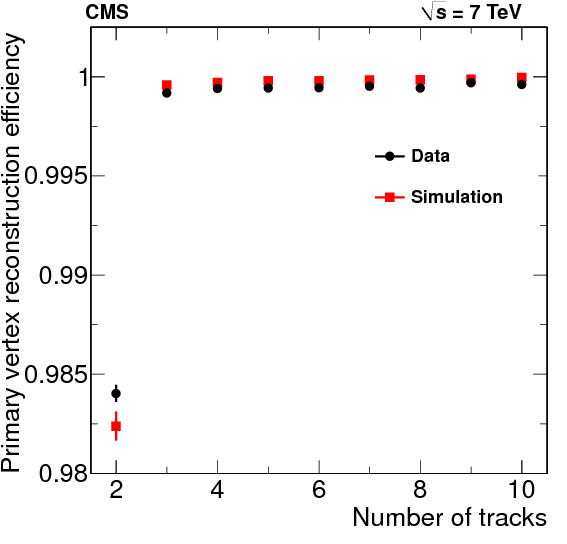
\includegraphics[width=.4\textwidth]{PV_eff}\hspace{1cm}
 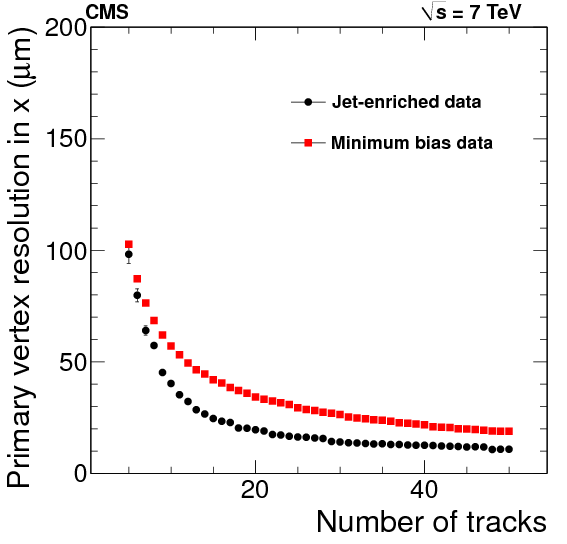
\includegraphics[width=.4\textwidth]{PV_res} 
 \caption{The primary vertex reconstruction efficiency (left) and resolution (right) as a function of the number of tracks associated to it.~\cite{Chatrchyan:2014fea}}
 \label{fig:PV}
\end{figure}

\subsection{Electron reconstruction}
\label{sec:electron_reconstruction}

\subsection{Muon reconstruction}
\label{sec:muon_reconstruction}

\subsection{Jet reconstruction}
\label{sec:jet_reconstruction}

\subsection{B-tagging}

\subsection{Missing transverse energy reconstruction}

\subsection{Particle flow}

\section{Simulation of the SIMP signal}


\clearpage
%\footnotesize
%\bibliographystyle{ieeetr}
%\bibliography{chapt8}
%\normalsize

\clearpage{\pagestyle{empty}\cleardoublepage}
